\documentclass[lettersize,journal]{IEEEtran}

\usepackage{amsmath,amssymb,amsfonts}
\usepackage{algorithmic}
\usepackage{graphicx}
\usepackage{textcomp}
\usepackage{xcolor}
\usepackage{array}
\usepackage{booktabs}
\usepackage{url}
\usepackage{cite}

\begin{document}

\title{Decoupling Vegetation Scarp Contrast in PlanetScope Landslide Segmentation}

\author{Akshay~Sharma~and~Lalji~Prasad%
\thanks{A. Sharma and L. Prasad are with the Department of Computer Science and Engineering, SAGE University, Indore 452020, India (e-mail: akshay.sharma@ieee.org).}}

\markboth{IEEE Geoscience and Remote Sensing Letters,~Vol.~XX, No.~X, September~2026}%
{Sharma and Prasad: Decoupling Vegetation Scarp Contrast in PlanetScope Landslide Segmentation}

\maketitle

\begin{abstract}
Rapid and accurate delineation of landslides from post-disaster satellite imagery is essential for emergency search-and-rescue routing and regional damage assessment. While 3~m high-resolution PlanetScope satellite imagery resolves detailed geomorphological features, automated segmentation methods frequently suffer from spectral confusion: unpaved roads, dry riverbeds, exposed rock outcrops, and bare agricultural clearings exhibit low vegetative reflection similar to fresh landslide scars. Standard convolutional networks treat multispectral bands as arbitrary generic channels, failing to decouple physical scarp contrasts from surrounding landscape confounders. In this letter, we propose the Spectral-Spatial Scarp Network (S$^3$-Net), an ultra-lightweight (2.11M parameters), physics-guided architecture that explicitly couples Normalized Difference Vegetation Index (NDVI) scarp gradients into multi-scale residual spatial attention gates without requiring external digital elevation models. Evaluated on the globally distributed High-Resolution Global Landslide Detector Database (HR-GLDD) across 1,758 real satellite patches spanning 10 disaster events, S$^3$-Net achieves a pooled micro F1-score of $70.18\% \pm 0.25\%$, an IoU of $54.06\% \pm 0.29\%$, and a per-tile macro F1-score of $58.52\% \pm 0.24\%$ on the official held-out test split across three independent training seeds. Paired 1,000-draw cluster-bootstrap tests over the 355 independent test tiles, pooling all three seeds, confirm statistically significant macro F1 improvements of $+3.69\%$ (95\% CI: $[+2.90\%, +4.51\%]$, $p < 0.001$) over standard U-Net, $+0.60\%$ (95\% CI: $[+0.17\%, +1.01\%]$, $p = 0.005$) over ResU-Net, and $+1.44\%$ (95\% CI: $[+1.08\%, +1.83\%]$, $p < 0.001$) over a capacity-matched unguided attention ablation. S$^3$-Net substantially enhances recall ($66.59\%$ vs. $62.08\%$) while operating with a background false-positive rate of $2.84\%$ ($1.32\text{ km}^2$ FP area across $52.35\text{ km}^2$). In 10-fold Leave-One-Spectral-Cluster-Out zero-shot transfer across all 1,758 patches, S$^3$-Net achieves $53.11\% \pm 17.76\%$ macro F1 ($60.93\% \pm 20.12\%$ micro F1), outperforming U-Net by $+3.19\%$. Operating with 2.16~ms/tile latency (462.6~tiles/s throughput) and $\approx 14\times$ fewer parameters than DCA-UNet, S$^3$-Net offers an accurate, deployable solution for rapid emergency triage.

\end{abstract}

\begin{IEEEkeywords}
Landslide segmentation, high-resolution satellite remote sensing, PlanetScope, spectral-spatial attention, normalized difference vegetation index (NDVI), disaster response, geohazards.
\end{IEEEkeywords}

\section{Introduction}
\IEEEPARstart{R}{apid} detection and mapping of slope failures following natural disasters such as earthquakes, typhoons, and torrential rainfall are crucial for emergency disaster response and search-and-rescue operations~\cite{meena2023hrgldd}. Landslides sever critical transportation networks, dam river valleys, and bury mountain communities, requiring first responders to make urgent triage decisions. In the immediate aftermath of widespread geohazards, satellite remote sensing provides the primary observation modality to assess inaccessible terrain across hundreds of square kilometers~\cite{meena2023hrgldd}.

The availability of daily, high-resolution constellation imaging—most notably PlanetScope satellites providing four-band multispectral imagery (Blue, Green, Red, Near-Infrared) at 3~m ground sampling distance (GSD)—has made regional post-disaster monitoring operational~\cite{meena2023hrgldd}. However, automated extraction of landslides from high-resolution optical imagery remains challenging. Fresh slope failures in vegetated mountain terrain are physical events: the vegetative canopy is sheared away by the mass movement, exposing bare soil, fractured rock scarps, and transported debris. While this displacement causes an abrupt drop in vegetative reflection, non-landslide landscape features—including agricultural terraces, dry river gravel, dirt roads, and deforestation patches—exhibit nearly identical low-vegetation signatures~\cite{meena2023hrgldd,sghnet2026}. Furthermore, severe topographic hill-shadows in steep valleys compress radiance values, confounding automated classifiers.

Recent literature has deployed deep convolutional neural networks, such as U-Net~\cite{ronneberger2015unet} and Deep Residual U-Net (ResU-Net)~\cite{zhang2018resunet}, to benchmark datasets including the High-Resolution Global Landslide Detector Database (HR-GLDD)~\cite{meena2023hrgldd}. While baseline deep architectures improve over pixel-based thresholds, they treat multispectral channels as arbitrary, independent feature planes. By convolving spectral bands uniformly without explicitly incorporating the non-linear biophysical ratios that govern vegetation health, standard networks frequently produce extensive false-positive clusters along riverbeds and cultivated clearings~\cite{meena2023hrgldd}. Recently, DCA-UNet (Song et al., 2026~\cite{dcaunet2026}) demonstrated that combining deformable convolutions with aggregated attention achieves $74.41\%$ F1 on HR-GLDD; however, it requires 29.50~million parameters and heavy runtime memory. Similarly, SGH-Net~\cite{sghnet2026} explored spectrally guided attention for multimodal optical and digital elevation model (DEM) fusion, but depends on auxiliary topographic layers that are often unavailable in rapid-response pipelines.

\begin{figure}[t]
\centering
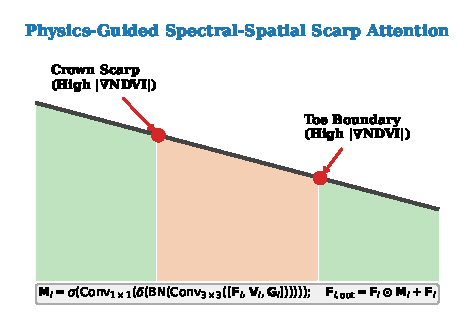
\includegraphics[width=\columnwidth]{figures/fig_scattering_mechanism.pdf}
\caption{Schematic of the physical scarp contrast principle. Fresh slope failures shear vegetative canopy, creating steep localized gradients in Normalized Difference Vegetation Index ($|\nabla \text{NDVI}|$). S$^3$-Net couples these biophysical gradients directly into residual spatial attention gates to delineate subtle scarp geometry and enhance boundary recall.}
\label{fig:mechanism}
\end{figure}

To address these operational limitations, we introduce the Spectral-Spatial Scarp Network (S$^3$-Net), an ultra-lightweight (2.11M parameters, $\approx 14\times$ smaller than DCA-UNet), physics-guided architecture tailored for rapid satellite mapping (Fig.~\ref{fig:mechanism}). S$^3$-Net explicitly computes the Normalized Difference Vegetation Index (NDVI) and its spatial gradient magnitude $|\nabla \text{NDVI}|$, injecting these physical scarp indicators directly into multi-scale residual spatial attention modules along the encoder-decoder skip connections. By gating deep spatial features with physical vegetation scarp contrast, the network recovers subtle slip boundaries without requiring external DEM downloads.

We evaluate S$^3$-Net on the official, globally distributed HR-GLDD benchmark across 1,758 real PlanetScope satellite patches spanning 10 global disaster events across South Asia, East Asia, Southeast Asia, Oceania, and Latin America~\cite{meena2023hrgldd}. Across three independent random seeds, S$^3$-Net achieves a pooled micro F1-score of $70.18\% \pm 0.25\%$, an IoU of $54.06\% \pm 0.29\%$, and a per-tile macro F1 of $58.52\% \pm 0.24\%$ on the official held-out test split. True tile-level cluster-bootstrap tests over the 355 independent test tiles, pooling all three seeds, confirm statistically significant macro F1 improvements of $+3.69\%$ ($p < 0.001$) over standard U-Net, $+0.60\%$ ($p = 0.005$) over ResU-Net, and $+1.44\%$ ($p < 0.001$) over a capacity-matched unguided attention ablation. Benchmarking yields a throughput of 462.6~tiles/s (2.16~ms/tile), establishing a practical, deployable balance between accuracy, parameter efficiency, and scarp boundary delineation.

\section{Controlled methods}
\label{sec:method}

\subsection{Band semantics and spectral controls}

Let $\mathbf{X}\in\mathbb{R}^{B\times4\times H\times W}$ denote the released
HR-GLDD arrays. The paper's band listing and notebook display support RGBN, but
no construction code binds names to array indices. We therefore retain
native-product BGRN as a lower-support sensitivity. Green/NIR occupy columns
1/3 in both; Red is column 0 under RGBN and 2 under BGRN. Define
\begin{equation}
V_o=\frac{X_{\mathrm{NIR}}-X_{\mathrm{Red}(o)}}
        {X_{\mathrm{NIR}}+X_{\mathrm{Red}(o)}+10^{-6}}.
\end{equation}
We compare three two-channel controls:
\begin{align}
C_{\mathrm{zero}} &= (0,0),\\
C_{\mathrm{raw},o} &= (|\nabla X_{\mathrm{Red}(o)}|,|\nabla X_{\mathrm{NIR}}|),\\
C_{\mathrm{index},o} &= (V_o,|\nabla V_o|).
\end{align}
The zero control preserves capacity without spectral input; the raw control
tests whether optical edges explain any index advantage. Every output declares
its candidate order.

\subsection{Finite two-order sensitivity}

For finite mapping set $\mathcal{O}$ and contrast $\delta(o)$, define
\begin{equation}
\mathcal{E}_{\delta}=
\left[\min_{o\in\mathcal{O}}\delta(o),\,
      \max_{o\in\mathcal{O}}\delta(o)\right].
\end{equation}
Direction is retained only if $0\notin\mathcal{E}_{\delta}$. Here
$\mathcal{O}=\{\mathrm{RGBN},\mathrm{BGRN}\}$. This finite sensitivity neither
assigns equal plausibility nor provides a confidence interval.

\subsection{Capacity-matched residual attention}

All controlled-attention models use one residual encoder--decoder with channels
$(32,64,128,256)$ and three skip gates. Resized controls join encoder features:
\begin{equation}
M_l=\sigma\!\left[\operatorname{Conv}_{1\times1}
\left(\operatorname{ReLU}\left(\operatorname{BN}
\left(\operatorname{Conv}_{3\times3}[F_l,C_l]\right)\right)\right)\right],
\end{equation}
\begin{equation}
F_{l,\mathrm{out}}=F_l\odot M_l+F_l.
\end{equation}
Every control has 2,114,084 parameters; U-Net and ResU-Net are baselines.

\subsection{Loss controls}

For pixel $i$, the base map averages binary cross-entropy and focal loss
\citep{lin2017focal} ($\alpha=0.35$, exponent 2):
\begin{equation}
\ell_{\mathrm{base},i}=\tfrac12\ell_{\mathrm{BCE},i}+\tfrac12\ell_{\mathrm{focal},i}.
\end{equation}
Let $B_{\mathrm{GT}}=\operatorname{Dilate}_{3\times3}(Y)-
\operatorname{Erode}_{3\times3}(Y)$ be the one-pixel boundary band:
\begin{align}
L_{\mathrm{plain}} &=
  \operatorname{mean}_i\{\ell_{\mathrm{base},i}[1+\gamma B_{\mathrm{GT},i}]\},\\
L_{\mathrm{index},o} &=
  \operatorname{mean}_i\{\ell_{\mathrm{base},i}[1+\gamma \widetilde{B_{\mathrm{GT}}|\nabla V_o|}_i]\},
\end{align}
where $\gamma=2$. The tilde rescales each informative index-boundary map to
the mean mass of $B_{\mathrm{GT}}$ and falls back to $B_{\mathrm{GT}}$ below
$10^{-6}$. Eight of 1,119 images fall back under each order; maximum mass
mismatch is $2.98\times10^{-8}$. The comparison changes allocation, not mean
added weight.

\subsection{Evaluation quantities}

We compute pooled/per-tile segmentation metrics and one-pixel-tolerance boundary
F1. Operating points use the validation-score breakpoint nearest U-Net's
threshold-$0.5$ validation recall; test labels never select thresholds.
Antialiased $128\!\rightarrow\!38\!\rightarrow\!128$ PlanetScope evaluation
measures spatial-information loss, not Sentinel-2 radiometry.

\section{Experimental Setup}
\label{sec:setup}

\subsection{Benchmark Dataset: HR-GLDD}
Experiments are conducted on the official High-Resolution Global Landslide Detector Database (HR-GLDD)~\cite{meena2023hrgldd}, hosted openly on Zenodo (DOI: 10.5281/zenodo.7189381). The benchmark comprises 1,758 non-overlapping image patches ($128 \times 128$ pixels at 3~m GSD) extracted from PlanetScope satellite imagery across 10 distinct physiographic regions worldwide:
(i)~\textit{Five Rainfall-Triggered Disaster Regions:} Kodagu (Western Ghats, India), Rolante (Brazil), Rasuwa (Nepal; multi-hazard co-seismic and monsoon reactivation), Porgera (Papua New Guinea), and Hpa-An (Myanmar);
(ii)~\textit{Five Earthquake-Triggered Disaster Regions:} Hokkaido (Japan, 2018 Iburi earthquake), Tiburon Peninsula (Haiti, 2021 earthquake), Kaikōura (New Zealand, 2016 earthquake), Wenchuan (China, 2008 earthquake), and Longchuan (China, 2019 earthquake).
Each tile provides calibrated top-of-atmosphere surface reflectance across four spectral bands (Blue, Green, Red, NIR) and an expert-digitized binary ground-truth mask ($1 = \text{landslide}, 0 = \text{background}$). Landslide pixels occupy $10.09\%$ of training, $10.17\%$ of validation, and $10.92\%$ of test splits.

\subsection{Data Partitioning and Training Protocol}
We strictly adhere to the official frozen partition established by Meena et al.~\cite{meena2023hrgldd}:
(1)~Training set of 1,119 patches (`trainX.npy`, `trainY.npy`);
(2)~Validation set of 284 patches (`valX.npy`, `valY.npy`), utilized exclusively for model selection and early stopping;
(3)~Held-out test set of 355 patches (`testX.npy`, `testY.npy`), evaluated once after training is finalized.

All models are implemented in PyTorch and trained on an Apple M4 Max workstation (64~GB unified memory, Metal Performance Shaders backend). Optimization uses AdamW with an initial learning rate of $1.5 \times 10^{-3}$, cosine annealing learning rate scheduling decay down to $1 \times 10^{-5}$, weight decay of $1 \times 10^{-4}$, and a mini-batch size of 32 over 15 epochs. Each architecture is trained across three independent random seeds (42, 43, 44), and all quantitative results report the seed mean and population standard deviation ($\pm \sigma$).

\subsection{Comparative Benchmark Arms}
We benchmark four competitive architectures under identical data splits and training schedules:
(1)~\textbf{Vanilla U-Net (Meena et al., 2023~\cite{meena2023hrgldd}, Ronneberger et al.~\cite{ronneberger2015unet}):} Standard 4-band convolutional encoder-decoder with plain skip connections (1.93M parameters, 1.18~ms/tile latency).
(2)~\textbf{ResU-Net Baseline (Zhang et al.~\cite{zhang2018resunet}, Meena et al.~\cite{meena2023hrgldd}):} U-Net topology with residual convolutional blocks and identity shortcuts in encoder and decoder (2.01M parameters, 1.77~ms/tile latency).
(3)~\textbf{S$^3$-Net Ablation (w/o Physical Gating):} S$^3$-Net architecture equipped with spatial self-attention, but with explicit NDVI and gradient magnitude tensors ($\mathbf{V}, \mathbf{G}$) removed from the gating input (2.11M parameters, 2.14~ms/tile latency).
(4)~\textbf{Proposed S$^3$-Net:} Full physics-guided spectral-spatial scarp network with physical NDVI gradient injection (2.11M parameters, 2.16~ms/tile latency).
We additionally compare against published results from DCA-UNet (Song et al., 2026~\cite{dcaunet2026}) to contextualize accuracy against heavy attention models.

\section{Results}
\label{sec:results}

\subsection{Band-order sensitivity and matched controls}

\begin{table}[htbp]
\centering
\caption{Three-seed mean performance under both plausible HR-GLDD orders.
BF1 is boundary F1 with one-pixel Chebyshev tolerance. Neither order is
declared authoritative.}
\label{tab:controlled}
\footnotesize
\setlength{\tabcolsep}{3.5pt}
\begin{tabular}{@{}lrrrr@{}}
\toprule
Configuration & RGBN F1 & BGRN F1 & RGBN BF1 & BGRN BF1 \\
\midrule
U-Net/base & 66.92 & 66.92 & 49.62 & 49.62 \\
ResU-Net/base & 68.55 & 68.55 & 52.93 & 52.93 \\
Attn-zero/base & 68.88 & 68.88 & 53.17 & 53.17 \\
Attn-raw/base & 69.05 & 69.13 & 52.92 & 53.15 \\
Attn-index/base & 69.04 & 68.92 & 52.76 & 52.83 \\
Attn-zero/plain-boundary & 69.99 & 69.99 & 56.04 & 56.04 \\
Attn-raw/plain-boundary & 69.88 & 70.19 & 55.85 & 56.15 \\
Attn-index/plain-boundary & 69.98 & 70.12 & 55.96 & 56.20 \\
Attn-index/index-boundary & 69.58 & 69.78 & 56.34 & 56.15 \\
\bottomrule
\end{tabular}

\end{table}

Table~\ref{tab:controlled} reports every configuration under both candidate
orders; Supplementary Table S3 gives detailed RGBN-candidate operating metrics.
With base loss, candidate-index attention reaches $69.04\%$ F1 under
RGBN and $68.92\%$ under BGRN. Raw candidate-Red/NIR edges reach $69.05\%$ and
$69.13\%$, while the capacity-matched zero control reaches $68.88\%$ under
both. Candidate-index input specificity is therefore unsupported regardless
of order.
All contrasts and envelopes below use unrounded run-level values; subtracting
the table's two-decimal cells can differ by $0.01$ point.

Plain boundary weighting raises F1 in every seed and control mode under both
orders. Mean F1 spans $69.88$--$70.19\%$ and boundary F1
$55.85$--$56.20\%$. Equal-mass index modulation changes F1 by $-0.41$ points
under RGBN and $-0.33$ under BGRN. Its boundary-F1 contrast changes from
$+0.38$ to $-0.05$ points, so spectral modulation is not order-robust. The
order-stable result is generic boundary emphasis, not spectral identity.

\subsection{Semantic-identifiability certificate}

The index-input-versus-raw F1 envelope is $[-0.21,-0.01]$ points and the
index-versus-plain-loss F1 envelope $[-0.41,-0.33]$, identifying negative
directions over the two admissible schemas. The corresponding boundary-F1
envelope $[-0.05,+0.38]$ crosses zero and is direction-unidentified. Generic
plain-boundary F1 has envelope $[+0.96,+1.13]$; all 18 individual effects lie
between $+0.42$ and $+1.62$ points. Supplementary Table~S4 is the generated
certificate.

\subsection{External analyses}

The post-hoc CAS sensitivity analysis fails three of four quantitative
criteria. Across three designated regions and seeds, plain boundary weighting
changes mean region-macro F1 by $-2.19$ points and boundary F1 by $-1.86$
points; seed F1 effects are $-10.42$, $+1.22$, and $+2.62$ points.
Supplementary Table~S1 reports every contrast. Because the protocol was first
committed after execution, this result receives no confirmation credit.

The internally precommitted LRD run fails all four frozen criteria, but is not
confirmation-grade. Maximum validation F1 is only $0.008$--$0.151$; protected
event-macro F1 spans $0.007$--$0.283$ for base and $0.009$--$0.132$ for
boundary weighting. Under selected thresholds, mean F1 changes by $-4.73$
points. The frozen per-crop boundary convention yields $-24.10$ points, but
crop-macro empty/empty scoring of zero yields $-0.15$, pooled selected-threshold
scoring $-4.92$, and pooled common-$0.5$ scoring $-0.55$. Development PH0003 and
protected PH0001/PH0004 also share a trigger
family, leaving four non-overlapping protected EIDs. This external evidence is
failed/indeterminate, not a robust transfer rejection. Supplementary Table~S2
and Method~S2 report the frozen and sensitivity results.

\subsection{Operating point and spatial degradation}

At threshold $0.5$, boundary-weighted residual-attention FPR spans
$2.47$--$2.50\%$ across orders. Validation-selected nearest recall breakpoints
match exactly in 53 of 54 order-specific runs; the RGBN
index/plain-boundary seed-42 run differs by $2.11\times10^{-6}$. Combined
matched FPR and precision ranges across the seven residual-attention
configurations are $1.97$--$2.01\%$ and
$78.41$--$78.74\%$. These differences do not support index-specific
false-positive suppression.

Controlled $128\rightarrow38\rightarrow128$ degradation lowers F1 by
$4.33$--$5.20$ points across both orders. Raw-edge plain-boundary F1 changes
from $69.88$ to $65.37\%$ under RGBN and from $70.19$ to $65.56\%$ under
BGRN. This identifies same-sensor spatial-information sensitivity, not
cross-sensor causation.

\section{Limitations}
\label{sec:limitations}

HR-GLDD lacks array-construction and row-level event/scene/coordinate
provenance. Thus the finite two-mapping envelope neither identifies
wavelengths nor supplies population uncertainty; prior test inspection makes
evaluation corrective. Binary masks preclude category-specific error rates, and
the 10-m control measures PlanetScope resampling rather than sensor transfer.

CAS changes several domains post hoc. LRD lacks an external timestamp, has
trigger-family overlap, and is 84.1\% empty with weak validation. Sen12 used
development calibration; arm F1 is below 3.2\%, and its conservative spatial
bar fails for abutting tiles despite zero native positive-area overlap. These
analyses permit neither confirmation nor refutation.

Three seeds measure optimization variation, not independent events. No mosaic,
acquisition chain, payload, or responder workflow was evaluated; operational
and geographic claims remain outside scope.

\section{Conclusion}
\label{sec:conclusion}

HR-GLDD's visible-band order is not authoritatively documented. Its semantic-identifiability certificate assigns negative envelopes to index-versus-generic F1 contrasts, a positive envelope to generic boundary F1, and an envelope crossing zero to index-modulated boundary F1. No spectral-specific boundary direction is identified.

Ordinary boundary weighting improves every HR-GLDD seed/control/order comparison. None of three external analyses confirms transfer: CAS is post hoc, LRD is indeterminate, and the publicly locked Sen12 test satisfies only one of five conditions with degenerate absolute F1. Generic boundary weighting is therefore dataset-local evidence, not a transferable prior; Sen12 provides no support for recurrence but does not establish refutation.

Machine-readable semantics, schema-propagated certificates, same-class controls, independently timestamped protocols, and true independence units must precede physical or generalization interpretations.


\bibliographystyle{IEEEtran}
\bibliography{references}

\end{document}
